\documentclass[../Report.tex]{subfiles}

\begin{document}

\chapter{Analysis and Design}

\section{Use case Diagram}
\begin{figure}[H]
    \centering
    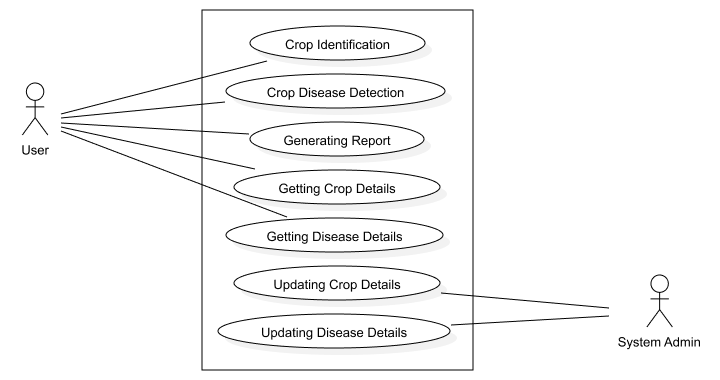
\includegraphics[width=0.8\linewidth]{images/usecase_2.png}
    \caption{Use Case Diagram}
    \label{fig:usecase}
\end{figure}

\section{Class Diagrams}
\begin{figure}[H]
    \centering
    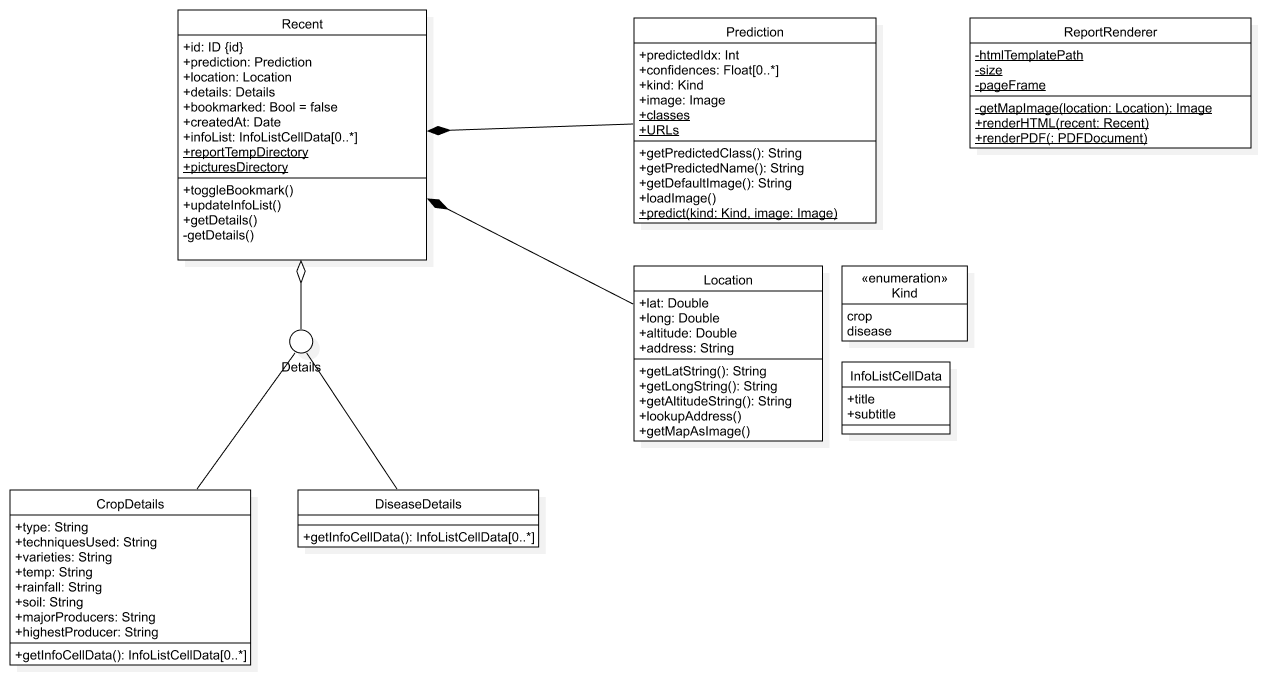
\includegraphics[width=0.8\linewidth]{images/class.png}
    \caption{Class Diagram}
    \label{fig:class}
\end{figure}

\section{Activity Diagrams}
\begin{figure}[H]
    \centering
    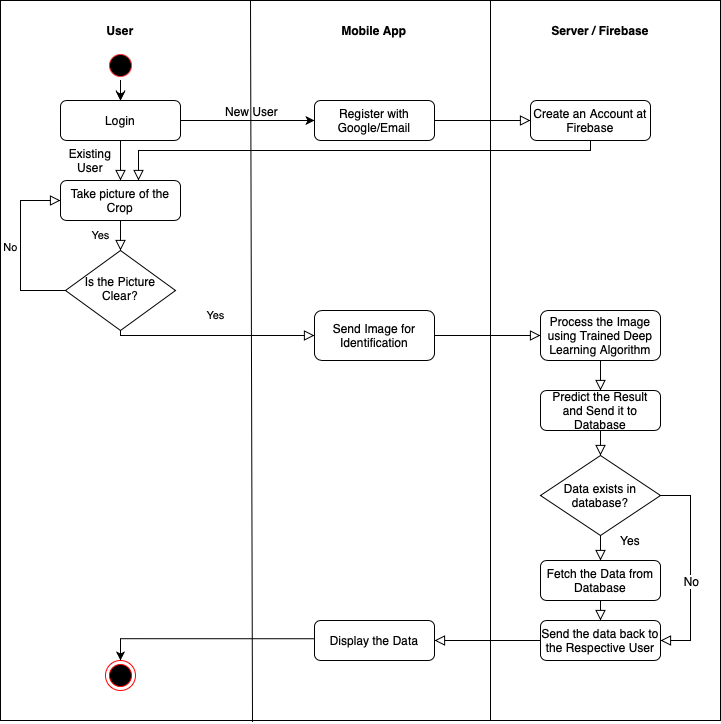
\includegraphics[width=\linewidth]{images/activity_crop.png}
    \caption{Activity Diagram for Crop Detection}
    \label{fig:activity_1}
\end{figure}

\begin{figure}[H]
    \centering
    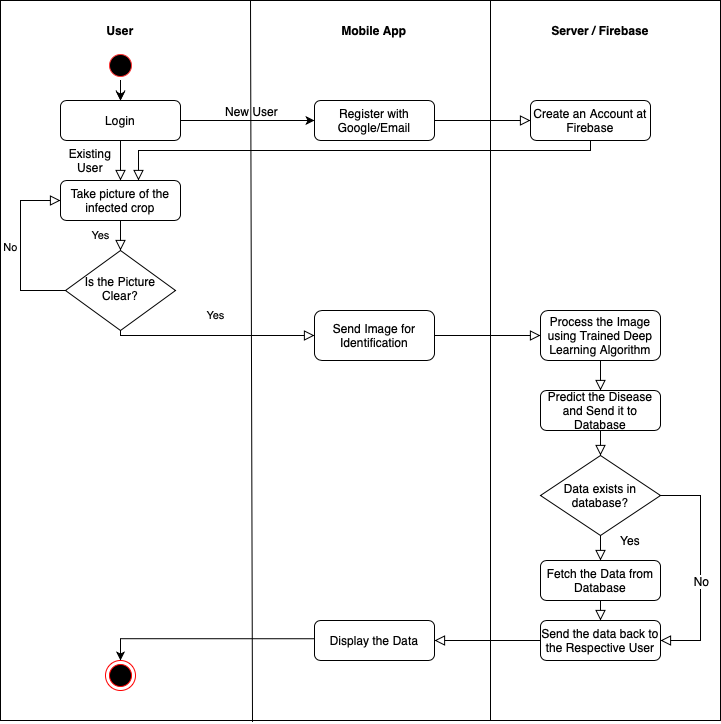
\includegraphics[width=\linewidth]{images/activity_disease.png}
    \caption{Activity Diagram for Disease Detection}
    \label{fig:activity_2}
\end{figure}

\section{Sequence Diagrams}
\begin{figure}[H]
    \centering
    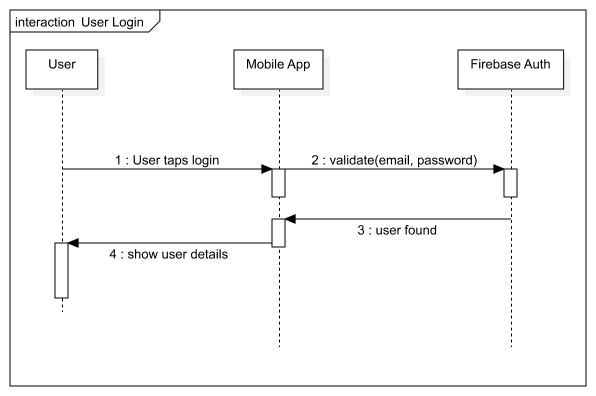
\includegraphics[width=0.95\linewidth]{images/seq_user_login.png}
    \caption{Sequence Diagram for User Login}
    \label{fig:seq_1}
\end{figure}

\begin{figure}[H]
    \centering
    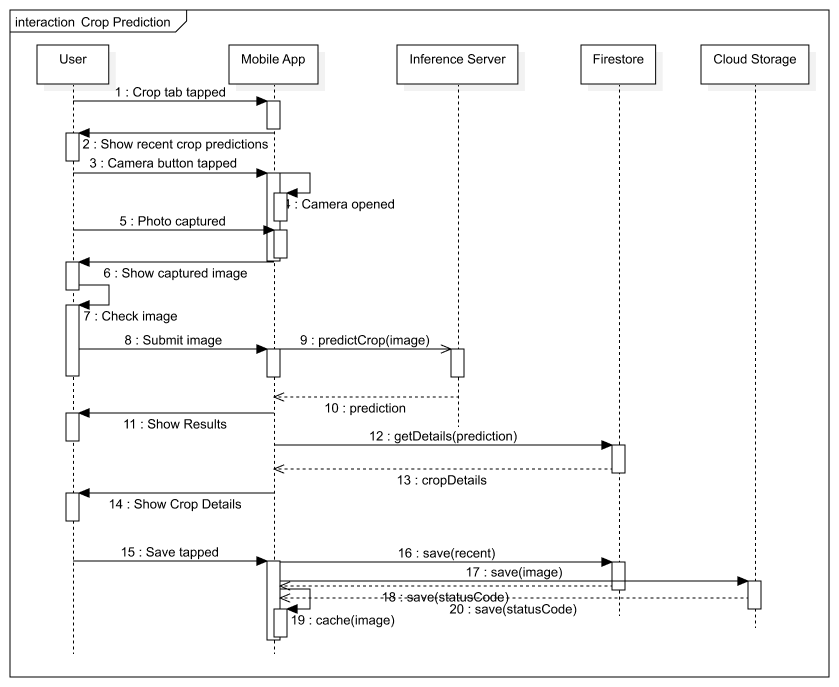
\includegraphics[width=0.95\linewidth]{images/seq_crop.png}
    \caption{Sequence Diagram for Crop Detection}
    \label{fig:seq_2}
\end{figure}

\begin{figure}[H]
    \centering
    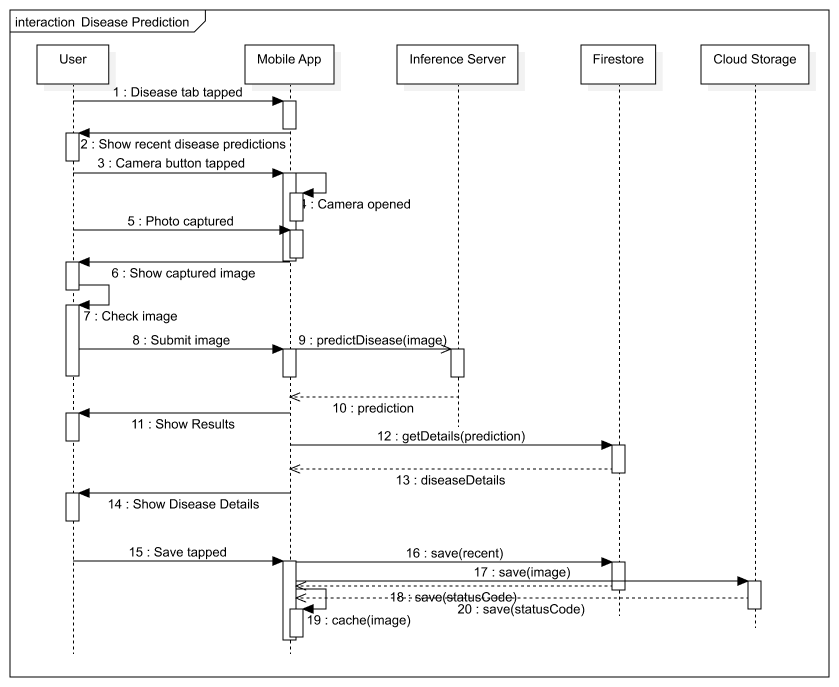
\includegraphics[width=0.95\linewidth]{images/seq_disease.png}
    \caption{Sequence Diagram for Disease Detection}
    \label{fig:seq_2}
\end{figure}

\section{System Architecture}
\begin{figure}[H]
    \centering
    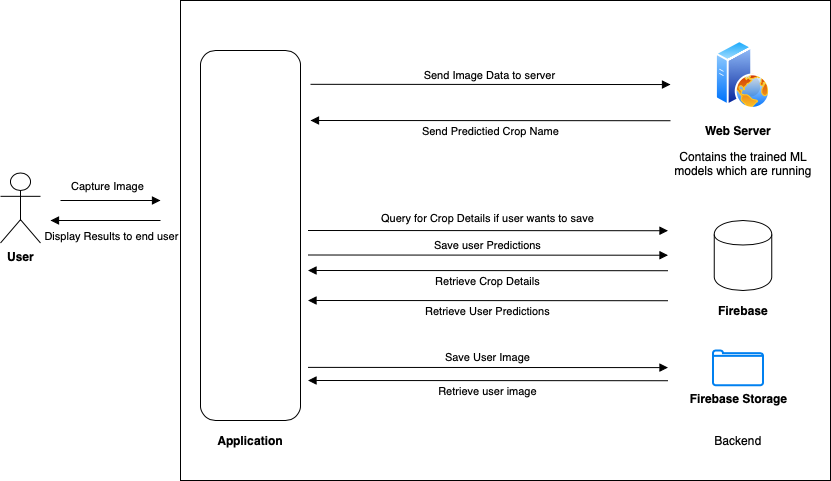
\includegraphics[width=0.95\linewidth]{images/architecture.png}
    \caption{App Architecture Diagram}
    \label{fig:architecture}
\end{figure}

\end{document}